% \documentclass[table]{beamer}
\documentclass[table,handout]{beamer}
\setbeameroption{show notes}
% \setbeameroption{hide notes}
% \setbeameroption{show only notes}
\usepackage{varwidth}

\newif\ifhide
\newif\ifpost
\newif\ifhideclicker

% \hidetrue
% \hideclickertrue
% \posttrue

\newcommand{\whiteout}[1]{\textcolor{white}{#1}}
% \newcommand{\whiteoutbox}[1]{\fcolorbox{white}{white}{\parbox{\dimexpr \linewidth-2\fboxsep-2\fboxrule}{\whiteout{#1}}}}
% \newcommand{\notebox}[1]{\fcolorbox{blue}{white}{\parbox{\dimexpr \linewidth-2\fboxsep-2\fboxrule}{#1}}}
\newcommand{\whiteoutbox}[1]{\fcolorbox{white}{white}{\parbox{\linewidth}{\whiteout{#1}}}}
\newcommand{\notebox}[1]{\fcolorbox{blue}{white}{\parbox{\linewidth}{#1}}}
\newcommand{\blankbox}[1]{\phantom{\varwidth{\linewidth}\whiteoutbox{#1}\endvarwidth}}
\newcommand{\blank}[1]{\phantom{\varwidth{\linewidth}#1\endvarwidth}}

\ifhide%
    \newcommand{\hmask}[1]{\blank{#1}}%
\else%
    \newcommand{\hmask}[1]{#1}%
\fi

\ifhide%
    \newcommand{\wout}[1]{\whiteout{#1}}%
\else%
    \newcommand{\wout}[1]{#1}%
\fi

\ifhide%
    \newcommand{\hignore}[1]{}%
\else%
    \newcommand{\hignore}[1]{#1}%
\fi

\ifpost%
    \newcommand{\nopost}[1]{}%
\else%
    \newcommand{\nopost}[1]{#1}%
\fi

\ifhideclicker%
    \newcommand{\clickerslide}[1]{\stepcounter{clickerQuestionCounter}%
        \begin{frame}[t]
            \textcolor{blue}{Q \arabic{clickerQuestionCounter}:}
        \end{frame}}
\else%
    \newcommand{\clickerslide}[1]{#1}%
\fi

\ifhide%
    \newcommand{\hidebox}[1]{\blank{#1}}%
\else%
    \newcommand{\hidebox}[1]{\notebox{#1}}%
\fi

\ifhide%
    \newcommand{\wbox}[1]{\whiteoutbox{#1}}%
\else%
    \newcommand{\wbox}[1]{\notebox{#1}}%
\fi

\ifhide%
    \newcommand{\nbox}[1]{\blankbox{#1}}%
\else%
    \newcommand{\nbox}[1]{\notebox{#1}}%
\fi

\ifhideclicker%
    \newcommand{\clickeranswer}[1]{#1}%
\else%
    \ifhide%
        \newcommand{\clickeranswer}[1]{#1}%
    \else%
        \newcommand{\clickeranswer}[1]{\textbf{\textcolor{blue}{#1}}}%
    \fi
\fi

\usepackage{beamerthemesplit}
% \usetheme{boxes}
\usetheme{Malmoe}
\usecolortheme{seahorse}
% \usecolortheme{seagull}
\usepackage{ifthen}
\usepackage{xspace}
\usepackage{multirow}
\usepackage{multicol}
\usepackage{booktabs}
\usepackage{xcolor}
\usepackage{wasysym}
\usepackage{comment}
\usepackage{hyperref}
\hypersetup{pdfborder={0 0 0}, colorlinks=true, urlcolor=blue, linkcolor=blue, citecolor=blue}
\usepackage{changepage}
\usepackage[compatibility=false]{caption}
\captionsetup[figure]{font=scriptsize, labelformat=empty, textformat=simple, justification=centering, skip=2pt}
\usepackage{tikz}
\usetikzlibrary{trees,calc,backgrounds}

\usepackage[bibstyle=joaks-slides,maxcitenames=3,mincitenames=1,backend=biber]{biblatex}

\newrobustcmd*{\shortfullcite}{\AtNextCite{\renewbibmacro{title}{}\renewbibmacro{in:}{}\renewbibmacro{number}{}}\fullcite}

\newrobustcmd*{\footlessfullcite}{\AtNextCite{\renewbibmacro{title}{}\renewbibmacro{in:}{}}\footfullcite}

% Make all footnotes smaller
% \renewcommand{\footnotesize}{\scriptsize}

\definecolor{myGray}{gray}{0.9}
\colorlet{rowred}{red!30!white}

\setbeamertemplate{blocks}[rounded][shadow=true]

\setbeamercolor{defaultcolor}{bg=structure!30!normal text.bg,fg=black}
\setbeamercolor{block body}{bg=structure!30!normal text.bg,fg=black}
\setbeamercolor{block title}{bg=structure!50!normal text.bg,fg=black}

\newenvironment<>{varblock}[2][\textwidth]{%
  \setlength{\textwidth}{#1}
  \begin{actionenv}#3%
    \def\insertblocktitle{#2}%
    \par%
    \usebeamertemplate{block begin}}
  {\par%
    \usebeamertemplate{block end}%
  \end{actionenv}}

\newenvironment{displaybox}[1][\textwidth]
{
    \centerline\bgroup\hfill
    \begin{beamerboxesrounded}[lower=defaultcolor,shadow=true,width=#1]{}
}
{
    \end{beamerboxesrounded}\hfill\egroup
}

\newenvironment{onlinebox}[1][4cm]
{
    \newbox\mybox
    \newdimen\myboxht
    \setbox\mybox\hbox\bgroup%
        \begin{beamerboxesrounded}[lower=defaultcolor,shadow=true,width=#1]{}
    \centering
}
{
    \end{beamerboxesrounded}\egroup
    \myboxht\ht\mybox
    \raisebox{-0.25\myboxht}{\usebox\mybox}\hspace{2pt}
}

\newenvironment{mydescription}{
    \begin{description}
        \setlength{\leftskip}{-1.5cm}}
    {\end{description}}

\newenvironment{myitemize}{
    \begin{itemize}
        \setlength{\leftskip}{-.3cm}}
    {\end{itemize}}

% footnote without a marker
\newcommand\barefootnote[1]{%
  \begingroup
  \renewcommand\thefootnote{}\footnote{#1}%
  \addtocounter{footnote}{-1}%
  \endgroup
}

% define formatting for footer
\newcommand{\myfootline}{%
    {\it
    \insertshorttitle
    \hspace*{\fill} 
    \insertshortauthor, \insertshortinstitute
    % \ifx\insertsubtitle\@empty\else, \insertshortsubtitle\fi
    \hspace*{\fill}
    \insertframenumber/\inserttotalframenumber}}

% set up footer
\setbeamertemplate{footline}{%
    \usebeamerfont{structure}
    \begin{beamercolorbox}[wd=\paperwidth,ht=2.25ex,dp=1ex]{frametitle}%
        % \Tiny\hspace*{4mm}\myfootline\hspace{4mm}
        \tiny\hspace*{4mm}\myfootline\hspace{4mm}
    \end{beamercolorbox}}

% remove navigation bar
\beamertemplatenavigationsymbolsempty

\makeatletter
    \newenvironment{noheadline}{
        \setbeamertemplate{headline}[default]
        \def\beamer@entrycode{\vspace*{-\headheight}}
    }{}
\makeatother

\newcounter{clickerQuestionCounter}
\ifhideclicker%
\newenvironment{clickerquestion}
{ \stepcounter{clickerQuestionCounter}
  \begin{enumerate}[Q \arabic{clickerQuestionCounter}:]\color{white} }
{ \end{enumerate} }
\else%
\newenvironment{clickerquestion}
{ \stepcounter{clickerQuestionCounter}
  \begin{enumerate}[Q \arabic{clickerQuestionCounter}:] }
{ \end{enumerate} }
\fi

\ifhideclicker%
\newenvironment{clickeroptions}
{ \begin{enumerate}[\begingroup\color{white} 1)\endgroup]\color{white} }
{ \end{enumerate} }
\else%
\newenvironment{clickeroptions}
{ \begin{enumerate}[\begingroup\color{red} 1)\endgroup] }
{ \end{enumerate} }
\fi


\tikzstyle{centered} = [align=center, text centered, font=\sffamily\bfseries]
\tikzstyle{skip} = [centered, inner sep=0pt, fill]
\tikzstyle{empty} = [centered, inner sep=0pt]
\tikzstyle{inode} = [centered, circle, minimum width=4pt, fill=black, inner sep=0pt]
\tikzstyle{tnode} = [centered, circle, inner sep=1pt]
\tikzset{
  % edge styles
  level distance=10mm,
  mate/.style={edge from parent/.style={draw,distance=3pt}},
  mleft/.style={grow=left, level distance=10mm, edge from parent path={(\tikzparentnode.west)--(\tikzchildnode.east)}},
  mright/.style={grow=right, level distance=10mm, edge from parent path={(\tikzparentnode.east)--(\tikzchildnode.west)}},
  % node styles
  male/.style={rectangle,minimum size=4mm,fill=gray!80},
  female/.style={circle,minimum size=4mm,fill=gray!80},
  amale/.style={male,fill=red},
  afemale/.style={female,fill=red},
}

\newcommand{\highlight}[1]{\textcolor{violet}{\textit{\textbf{#1}}}}
\newcommand{\super}[1]{\ensuremath{^{\textrm{\sffamily #1}}}}
\newcommand{\sub}[1]{\ensuremath{_{\textrm{\sffamily #1}}}}
\newcommand{\dC}{\ensuremath{^\circ{\textrm{C}}}}
\newcommand{\tb}{\hspace{2em}}
\providecommand{\e}[1]{\ensuremath{\times 10^{#1}}}
\newcommand{\myHangIndent}{\hangindent=5mm}

\newcommand{\spp}[1]{\textit{#1}}

\newcommand\mybullet{\leavevmode%
\usebeamertemplate{itemize item}\hspace{.5em}}

\makeatletter
\newcommand*{\rom}[1]{\expandafter\@slowromancap\romannumeral #1@}
\makeatother

\newcommand{\blankslide}{{\setbeamercolor{background canvas}{bg=black}
\setbeamercolor{whitetext}{fg=white}
\begin{frame}<handout:0>[plain]
\end{frame}}}

\newcommand{\whiteslide}{
\begin{frame}<handout:0>[plain]
\end{frame}}

\newcommand{\f}[1]{\ensuremath{F_{#1}}}
\newcommand{\x}[1]{X\ensuremath{^{#1}}}
\newcommand{\y}[1]{Y\ensuremath{^{#1}}}

% Population growth macros
\newcommand{\popsize}[1]{\ensuremath{N_{#1}}}
\newcommand{\popgrowthratediscrete}[1]{\ensuremath{\lambda_{#1}}}
\newcommand{\popgrowthrate}[1]{\ensuremath{r_{#1}}}
\newcommand{\ptime}{\ensuremath{t}\xspace}

\tikzset{hide on/.code={\only<#1>{\color{white}}}}
\tikzset{
    invisible/.style={opacity=0},
    visible on/.style={alt={#1{}{invisible}}},
    alt/.code args={<#1>#2#3}{%
        \alt<#1>{\pgfkeysalso{#2}}{\pgfkeysalso{#3}}
        % \pgfkeysalso doesn't change the path
    },
}

% \bibliography{../bib/references}
\bibliography{references}
\author[J.\ Oaks]{
    %Jamie R.\ Oaks\inst{1}
    Jamie R.\ Oaks
}
\institute[BIOL 180]{
    \inst{}%
        BIOL 180: Introductory Biology
}



\title[Mutation \& Drift]{Mutation and Drift}
% \date{\today}
\date{April 27, 2015}

\begin{document}

\begin{noheadline}
\maketitle
\end{noheadline}

\nopost{
\begin{noheadline}
\begin{frame}[c]
    \vspace{-6mm}
    \begin{center} 
        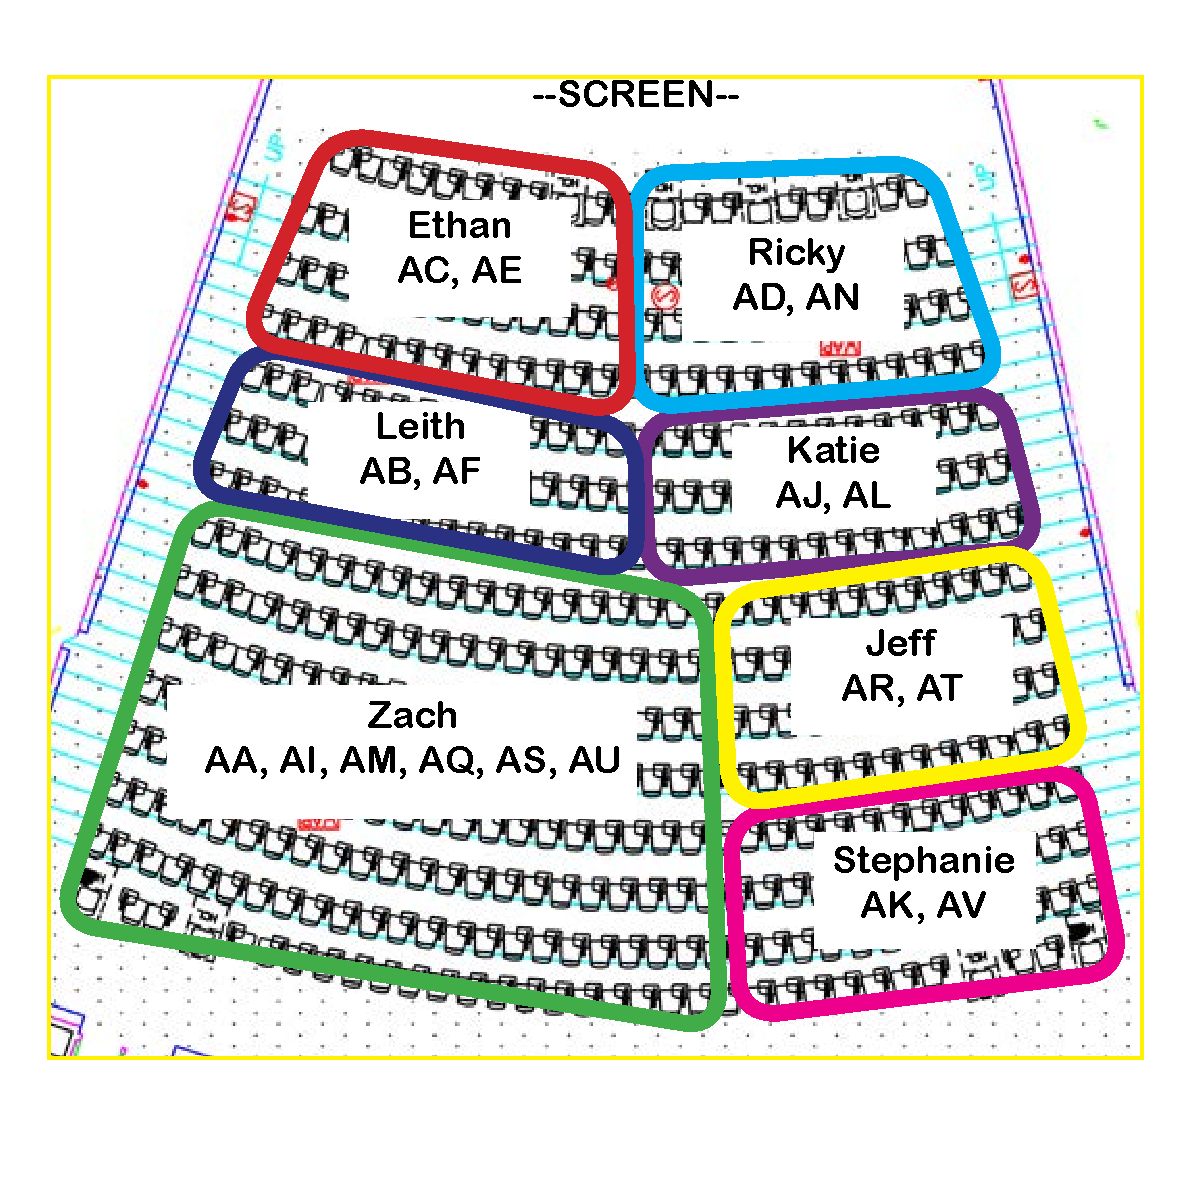
\includegraphics[height=1.2\textheight]{../images/seating-chart.pdf}
    \end{center}
\end{frame}
\end{noheadline}
}

\clickerslide{
\begin{noheadline}
\begin{frame}
    \begin{clickerquestion}
        \item
            In the media, people are talking about how the Ebola virus will
            evolve airborne transmission in order to spread to new hosts more
            efficiently. What is wrong with this reasoning?

        \begin{clickeroptions}
            \item Evolution by natural selection is not progressive; it is
                random.
            \item Adaptations are favored because they ensure the survival of
                the species.
            \item \clickeranswer{Natural selection can only act on existing
                    heritable variation, and mutations are random with respect
                    to fitness.}
            \item Nothing; airborne transmission would increase fitness, and so
                natural selection will cause it to evolve.
        \end{clickeroptions}
    \end{clickerquestion}
\end{frame}
\end{noheadline}
}

\begin{noheadline}
\begin{frame}
\frametitle{Today's issues:}
\tableofcontents[subsectionstyle=hide]
\end{frame}
\end{noheadline}

\section{How does mutation cause changes in allele frequencies?}

\subsection{How often do mutations occur?}

\begin{frame}
    \frametitle{Data from \textit{Arabidopsis thaliensis}}
    \begin{itemize}
        \item<1-> \textit{A. thaliensis} is a diploid mustard that can self.

        \item<2-> Experimental design: Start with 1 individual; let it grow in
            optimum conditions (soil, light, moisture, space) and
            self-fertilize.

        \item<3-> Choose 1 seed at random to be the next generation \ldots let
            it grow, choose 1 seed at random etc. \ldots total of 30
            generations \ldots 5 lines (replicates)

        \item<4-> Sequence the entire genome at generations 1 and 30
    \end{itemize}
\end{frame}

\begin{frame}[t]
    \frametitle{Data from \textit{Arabidopsis thaliensis}}
    \begin{adjustwidth}{-1.5em}{-1.5em}
        \vspace{-3mm}
    \begin{itemize}
        \item<1-> Estimated an average of  $7 \times 10^{-9}$ mutations per base
            per generation

        \item<2-> Haploid genome size is $\approx 1.35 \times 10^8$ bases

        \item<3-> Average gene size is $\approx 3000$ bases
    \end{itemize}

    \begin{enumerate}
        \item<4-> What is the average number of mutations per haploid genome per
            generation?

            \nbox{$0.95 = (7 \times 10^{-9} mutations/base/generation)(1.35 x
                10^8 bases)$}

            \vspace{3mm}
        \item<4-> What is average number of mutations per seed per generation?

            \nbox{$0.95 \times 2$}

            \vspace{3mm}
        \item<4-> What is the average number of mutations per gene copy per
            generation?

            \nbox{\scriptsize $2.1 \times 10^{-5} mutations/gene = (7 \times 10^{-9}
                mutations/base/generation)(3000 bases)$}
    \end{enumerate}
    \note[item]{Similar experiment with \textit{C.\ elegans}; rate is
        $\approx$2.5x higher}
    \end{adjustwidth}
\end{frame}

\begin{frame}[t]
    \frametitle{Data from \textit{Arabidopsis thaliensis}}
    \begin{adjustwidth}{-1.5em}{-1.5em}
    \begin{itemize}
        \item You expect $2.1 \times 10^{-3} \%$ of gene copies to be a new
            allele each generation.

        \item How many generations would it take to expect a 1\% change in
            allele frequency for a given gene?
            
            \nbox{$476 generations \approx 0.01 / 2.1 \times 10^{-5}$}
    \end{itemize}
    \end{adjustwidth}
\end{frame}

\begin{frame}
    Take-home messages:

    \begin{itemize}[<+->]
        \item By itself (i.e., all other HW conditions are satisfied), mutation
            does not change allele frequencies very much.

        \item However, mutation constantly creates heritable variation in all
            populations in every generation.
    
        \item It is the source of variation on which selection, drift, and
            migration can act.
    \end{itemize}

\end{frame}

\begin{frame}
    \begin{clickerquestion}
        \item Mutation is sometimes called the ultimate source of genetic
            variation. Why is this accurate?
        \begin{clickeroptions}
            \item Mutation is random with respect to fitness.
            \item \clickeranswer{Meiosis creates new genotypes, but only
                    mutation creates new alleles.}
            \item Mutations do not blend together (genes are particulate).
            \item It creates new genotypic variation.
        \end{clickeroptions}
    \end{clickerquestion}
\end{frame}

\section{How do mutations affect fitness?}

\begin{frame}
    \frametitle{Experiment on \emph{C. elegans}}
    \begin{adjustwidth}{-1.5em}{-1.5em}

    Suzanne Estes and colleagues maintained lines of \emph{C. elegans} for many
    generations in the lab:

    \begin{description}
        \item[Control lines] Large populaions; allowed for selection.
        \item[Experimental lines] Prevented selection; mutations accumulate.
    \end{description}

    \begin{center}
    \begin{tikzpicture}
    [scale=0.38,auto=left,every node/.style={circle}]%,fill=blue!20}]
      \node [skip](xy) at (0,0) {};
      \node [empty](x) at (14,0) {};
      \node [empty](y) at (0,10) {};
      \node [empty, label=below: {\sffamily Time}](xl) at (7.5,0.5) {};
      \node [empty, label=left: {\sffamily Lifespan}](yl) at (0,5) {};
      \node [empty](k1l) at (-16, 8) {};
      \node [empty, label=right: {\sffamily Control lines}](k1r) at (-14, 8) {};
      \node [empty](k2l) at (-16, 3) {};
      \node [empty, label=right: {\sffamily Experimental lines}](k2r) at (-14, 3) {};
    
      \foreach \from/\to in {xy/x,xy/y,k1l/k1r}
        \draw [thick] (\from) -- (\to);
      \foreach \from/\to in {k2l/k2r}
        \draw[thick,dashed] (\from) -- (\to);
    
    \end{tikzpicture}
    \end{center}
    \end{adjustwidth}
    \note[item]{\textit{C.\ elegans} reproduce throughout lifetime, so lifespan
        is a good measure of fitness}
\end{frame}

\section{How does genetic drift change allele frequencies?}

\begin{frame}[t]
    ``Drift happens'': Chance variation in reproductive success (i.e., sampling
    error or ``luck'').
    
    \vspace{0.5cm}
    Experiment 1: Starting population size = 2

    \begin{table}%[htbp]
        \centering
        \begin{tabular}{ p{2.5cm} p{2cm} p{2.5cm} }
             Mom: $A_{H}A_{T}$ & & Dad: $A_{H}A_{T}$ \\
             & & \\
             $fr(A_{H})=$ & & $fr(A_{T})=$ \\
              & & \\
             Kids & & \\
             1: & & 2: \\
             3: & & 4: \\
             5: & & 6: \\
             & & \\
             $fr(A_{H})=$ & & $fr(A_{T})=$ \\
        \end{tabular}
    \end{table}
\end{frame}

\begin{frame}
    Experiment 2: Starting population size $\approx 800$

    \begin{table}%[htbp]
        \centering
        \begin{tabular}{ p{2.5cm} p{2cm} p{2.5cm} }
             Mom: $A_{H}A_{T}$ & & Dad: $A_{H}A_{T}$ \\
             $fr(A_{H})=$ & & $fr(A_{T})=$ \\
        \end{tabular}
    \end{table}

    Flip a coin or use 2 little pieces of paper (one with ``H'' and one with
    ``T'') to make your offspring!

    \vspace{0.5cm}
    Clickers:
    \begin{enumerate}
        \item $A_{H}A_{H}$
        \item $A_{H}A_{T}$
        \item $A_{T}A_{T}$
    \end{enumerate}

    \begin{table}%[htbp]
        \centering
        \begin{tabular}{ p{2.5cm} p{2cm} p{2.5cm} }
             $fr(A_{H})=$ & & $fr(A_{T})=$ \\
        \end{tabular}
    \end{table}

\end{frame}

\begin{frame}
    Punchlines:

    \begin{itemize}
        \item Does drift have a stronger affect on allele frequencies in small
            or large populations?
            \nbox{Small populations; sampling fewer gametes each generation
                and so will have larger changes in allele frequencies due to
                chance.}

        \item What happens when drift continues, generation after generation
            (especially in small populations)?
            \nbox{alleles will drift to fixation or loss}
    \end{itemize}
\end{frame}

\begin{frame}
    Many events can cause drift

    \begin{itemize}
        \item Airplanes crash

            \nbox{Bad luck \ldots alleles don't get passed on}

        \item When the Grants were working in the Galapagos, they observed a
            small group of \emph{Geospiza magnirostris} arrive on Daphne Major
            and start a new population

            \nbox{Only a few individuals---likely dramatic shifts in allele
                frequencies compared to source population}

        \item When Europeans brought smallpox and measles to North America, up
            to 90\% of Native Americans in some communities died

            \nbox{Alleles of immune system genes under intense selection,
                but alleles for independent genes change dramatically in
                frequency just due to chance}
    \end{itemize}
\end{frame}

\begin{frame}
    \begin{clickerquestion}
        \item
            Many mutations do not change the phenotype (e.g., a change from AAT
            to AAC in DNA still means a leucine will be in the gene product).
            But many mutations like this have increased to fixation in human
            and other populations. How?

        \begin{clickeroptions}
            \item Mutation---the same AAT-AAC mutation occurred in many individuals.
            \item Selection---leucine is favored.
            \item \clickeranswer{Drift---the ``AAC allele'' got lucky.}
            \item Gene flow---individuals with the AAC allele moved in;
                individuals with the AAT allele moved out.
            \item Nonrandom mating---individuals with high leucine content tend
                to mate together.
        \end{clickeroptions}
    \end{clickerquestion}
\end{frame}

\begin{frame}
    \begin{clickerquestion}
        \item
            Consider the following experiment: 100 fruit fly populations in the
            lab, each consisting of 4 females and 4 males. In each starting
            population, alleles $A_1$ and $A_2$ are at frequency 0.5.
 
        \begin{itemize}
            \item Randomly pick 4 female and 4 male offspring to breed and form
                the next generation in each population. Note: this is a VERY
                TINY population. 

            \item Repeat for a total of 16 generations, in each of the 100
                populations.

            \item Plot the number of populations (total of 100) that have
                allele $A_1$ at various frequencies, from 0 (lost) to 1.0
                (fixed). 

            \item Which of the following graphs predicts the result correctly? 
        \end{itemize}

    \end{clickerquestion}
\end{frame}

\begin{frame}
    \centering{
        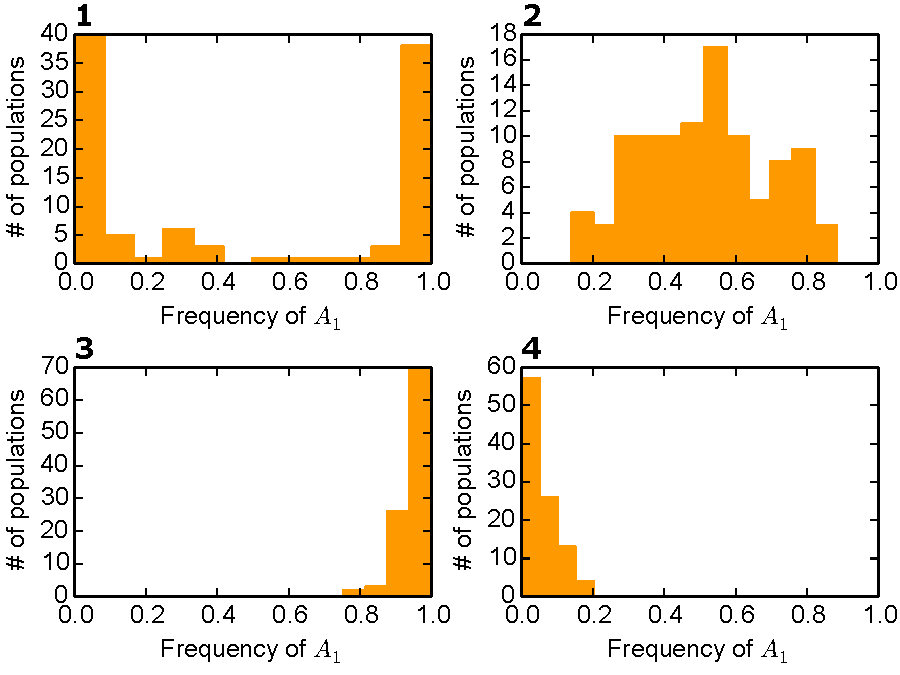
\includegraphics[width=0.95\textwidth]{../images/allele-freq-clicker-histograms.pdf}}

    \nbox{\scriptsize Correct answer is 1}
\end{frame}

\begin{frame}[t]
    \frametitle{Consequences of genetic drift}
    \begin{enumerate}
        \item With respect to fitness, drift \ldots

            \nbox{is random}

            \vspace{1cm}
        \item With respect to genetic varition, drift \ldots

            \nbox{will reduce genetic varition over time}

            \vspace{1cm}
        \item Why is drift a concern for endangered species?

            \nbox{Drift is pronounced in small populations and can reduce
                genetic varition}
    \end{enumerate}
\end{frame}


\end{document}


